\paragraph{QuizziPedia::Front-End::Controllers::RegistrationManagementController}
\begin{figure} [ht]
	\centering
	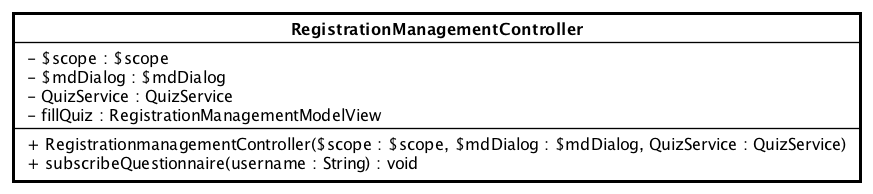
\includegraphics[scale=0.45]{UML/Classi/Front-End/QuizziPedia_Front-end_Controller_RegistrationManagementController.png}
	\caption{QuizziPedia::Front-End::Controllers::RegistrationManagementController}
\end{figure} \FloatBarrier
\begin{itemize}
	\item \textbf{Descrizione}: questa classe permette di gestire le iscrizione degli utenti ai questionari;
	\item \textbf{Utilizzo}: fornisce le funzionalità di iscrizione ad un questionario;
	\item \textbf{Relazione con altre classi}:
	\begin{itemize}
		\item \textit{IN} \texttt{RegistratioManagementModelView}: ; 
		\item \textit{OUT} \texttt{QuizService}: questa classe permette di ottenere i dati di un quiz tramite delle parole chiave inserite dall'utente nella barra di ricerca;
	\end{itemize}
	\item \textbf{Attributi}:
	\begin{itemize}
		\item \texttt{-} \texttt{\$scope: \$scope} \\
		Campo dati contenente un riferimento all’oggetto \$scope creato da \textit{Angular\ped{G}}, viene utilizzato come mezzo di comunicazione tra il controller e la view. Contiene gli oggetti che definiscono il model dell’applicazione;
		\item \texttt{-} \texttt{\$mdDialog: \$mdDialog} \\
		Campo dati contenente un riferimento al servizio della libreria \textit{Material for Angular\ped{G}} che permette di creare delle componenti a popup;
		\item \texttt{QuizService: QuizService}\\ parametro che permette di ottenere, tramite il service, la lista di tutte le domande presenti nel quiz;
		\item \texttt{+} \texttt{fillQuiz: RegistrationManagementModelView} \\
		Oggetto di tipo \texttt{RegistrationManagementModelView}. All'interno di esso sono presenti le variabili e i metodi necessari per il \textit{Two-Way Data-Binding\ped{G}} tra la view \texttt{RegistrationManagemenView} e il controller \texttt{RegistrationManagemenController};
	\end{itemize}
	\item \textbf{Metodi}:
	\begin{itemize}
		\item \texttt{RegistrationmanagementController(\$scope: \$scope, \$mdDialog: \$mdDialog, QuizService: QuizService)}: \\Metodo costruttore della classe. \\
			\textbf{Parametri}:
			\begin{itemize}
					\item \texttt{-} \texttt{\$scope: \$scope} \\
					Campo dati contenente un riferimento all’oggetto \$scope creato da \textit{Angular\ped{G}}. Viene utilizzato come mezzo di comunicazione tra il controller e la view. Contiene gli oggetti che definiscono il viewmodel e il model dell’applicazione;
					\item \texttt{-} \texttt{\$mdDialog: \$mdDialog} \\
					Campo dati contenente un riferimento al servizio della libreria \textit{Material for Angular\ped{G}} che permette di creare delle componenti a popup;
					\item \texttt{-} \texttt{QuizService: QuizService}: parametro che permette di ottenere, tramite il service, la lista di tutte le domande presenti nel quiz; 
			\end{itemize}
		\item \texttt{subscribeQuestionnaire(username: String): void} \\ Metodo che permette l'iscrizione ad un questionario. Richiama la funzionalità del QuizService. \\
		\textbf{Parametri}:
		\begin{itemize}
			\item \texttt{username: String}: parametro che indica l'utente da iscrivere al questionario.
		\end{itemize}
	\end{itemize}
\end{itemize}

